\section{Research Plan}

\subsection{Task 1: Understanding HSRN researchers’ needs and behaviors}

\begin{figure}[t]
    \centering
    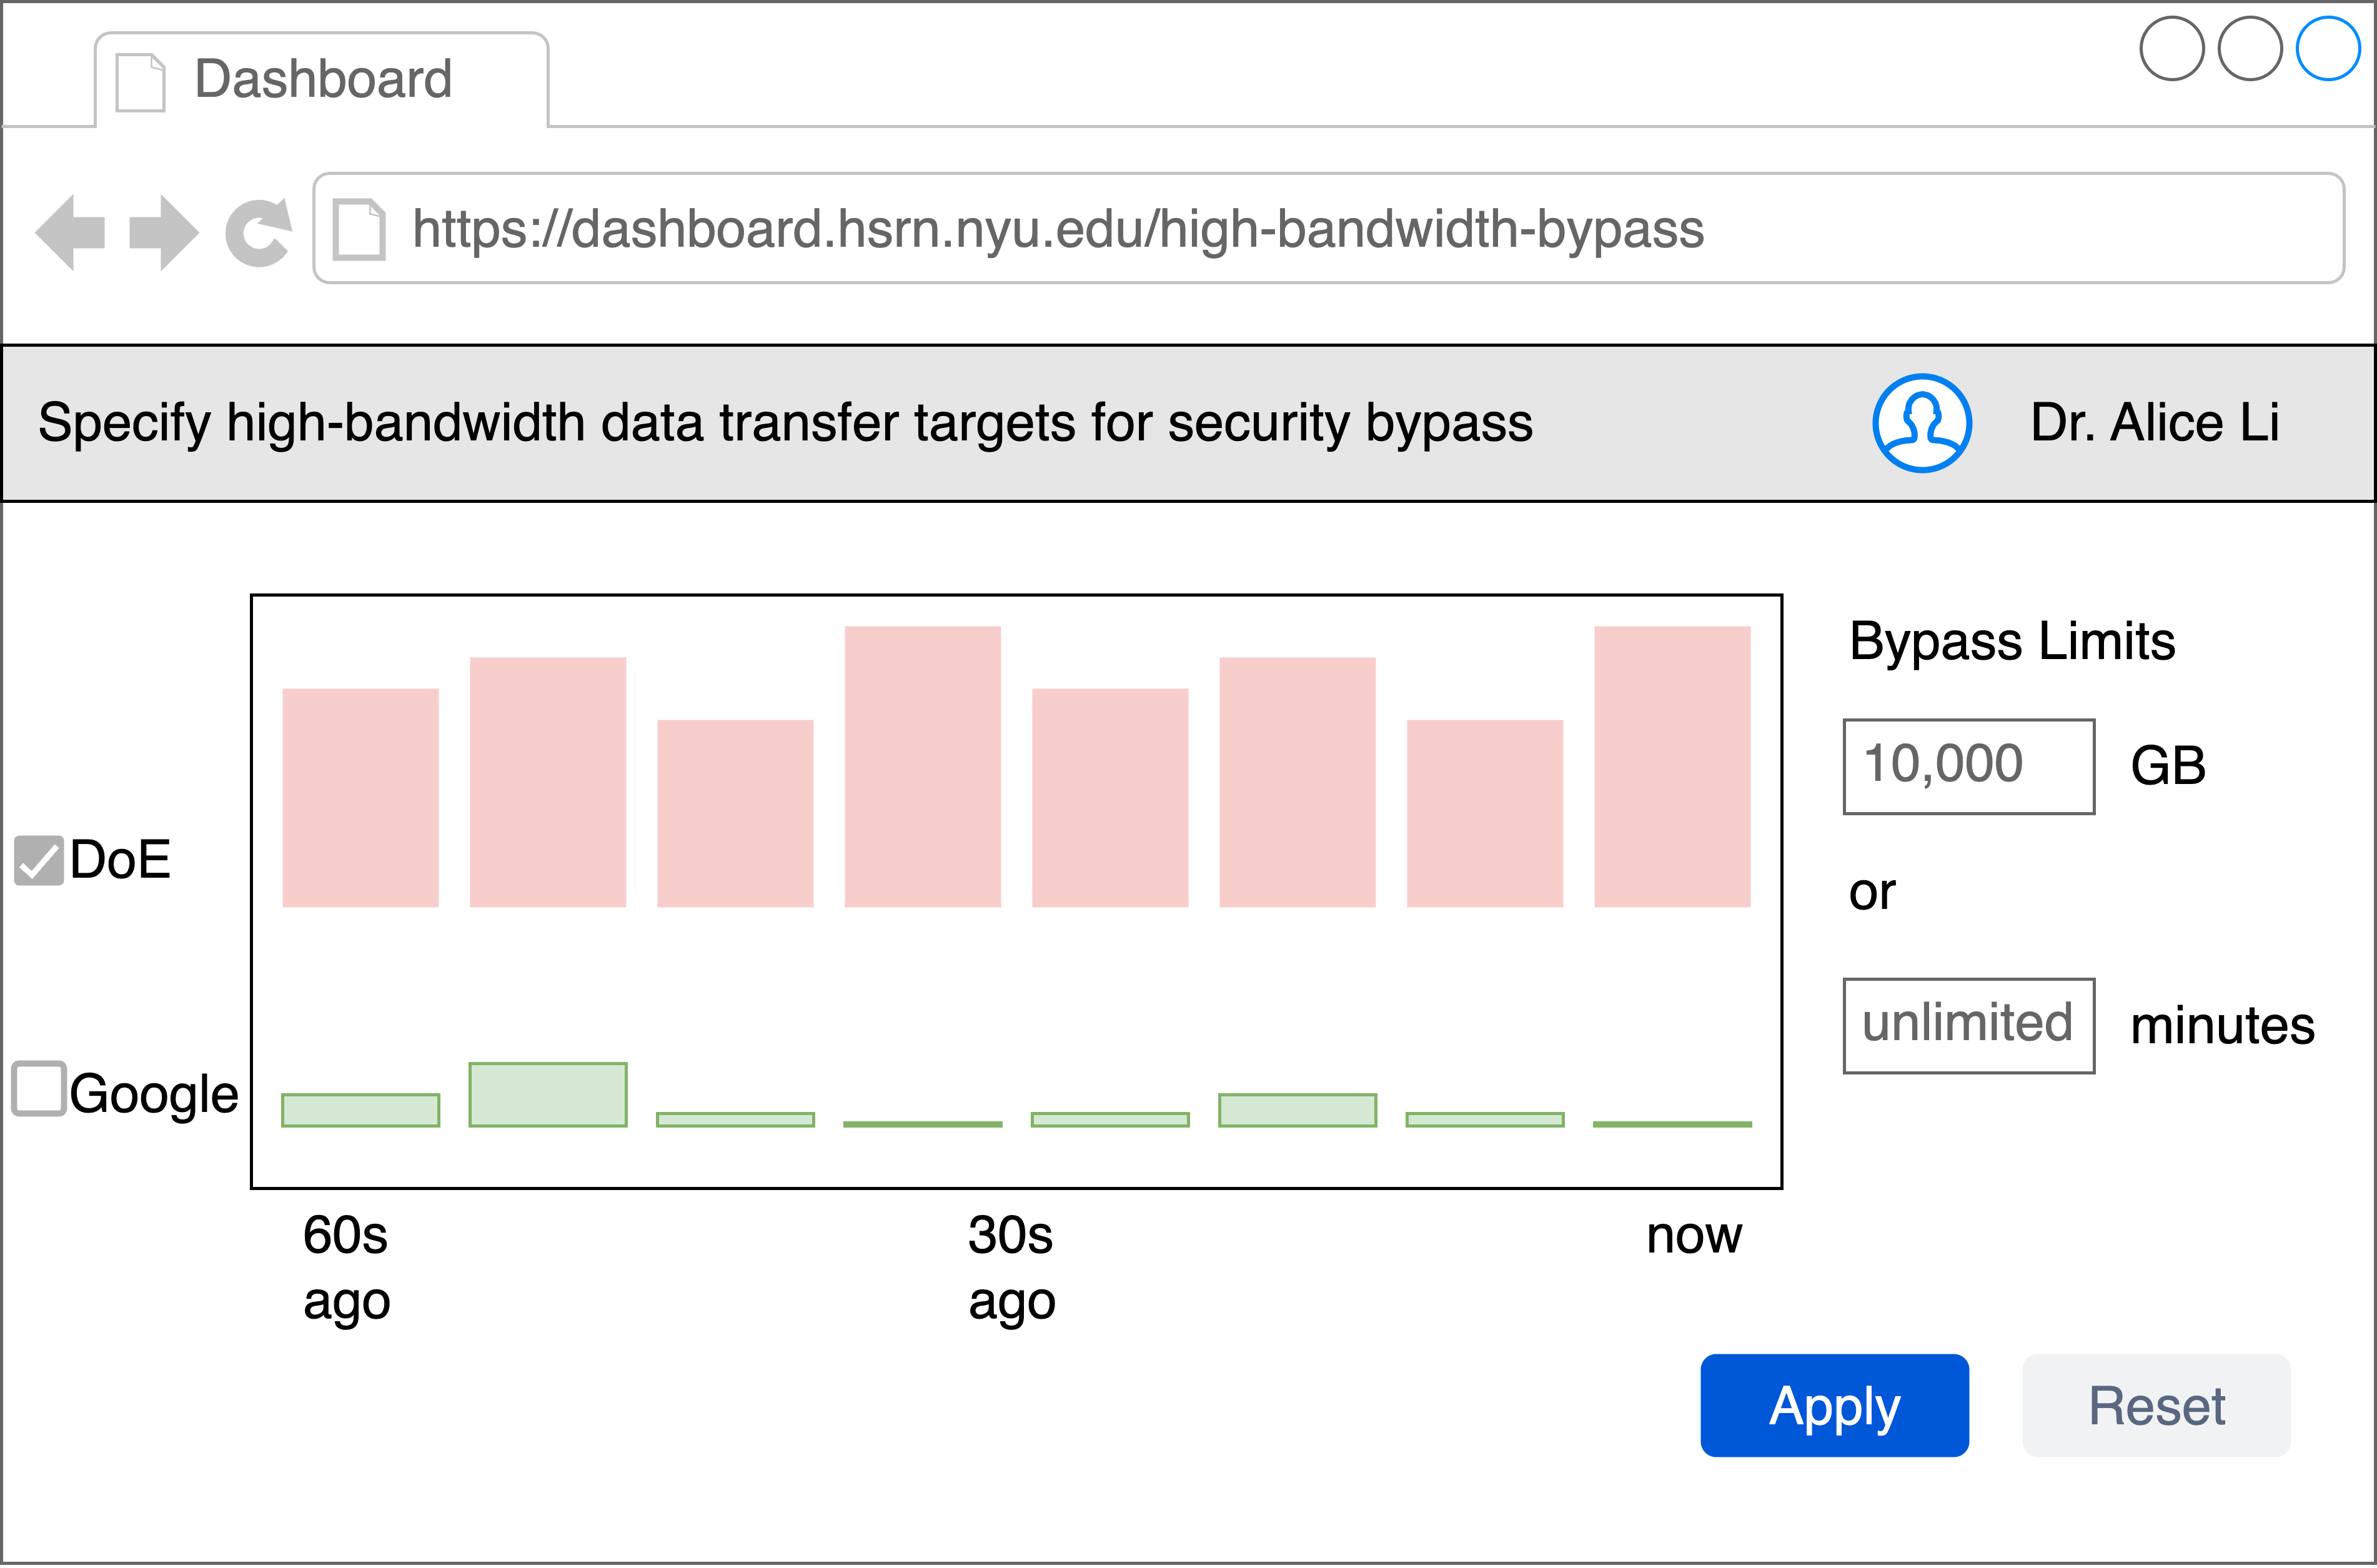
\includegraphics[width=0.5\linewidth]{figures/dashboard.png}
    \caption{A sample of the dashboard's user interface.}
    \label{fig:dashboard}
\end{figure}


Understanding researchers’ needs help us design the user-facing components (UI/UX).

Understanding their behaviors help us make automated decisions to help them (especially in Task 2).

Task 1a: Understanding researchers’ needs through user studies

Understanding concerns. Through surveys and semi-structured interviews, we plan to understand how they are currently using the HSRN and their experience with the network administrators.

Co-designing UI/UX. We plan to co-design sessions in focus groups to make preliminary designs on what the dashboard looks like and the proposed user interactions. Make sure that our design is a part of their workflow.

Understand how they want to express blessed destinations or network behaviors. end-users of open scientific infrastructure may consider security processes valuable only insofar as they do not slow or otherwise impede their research

Understand qualitatively what kind of network traffic they send. Elephant flows, or latency sensitive flows, presumably depending on what kind of experiment or research work they do.

Preliminary work. Inspector dashboard, CHI paper dashboard

Expected outcome.

// From: Jeremy
-An open source tool to monitor,visualize and manage security and data transmission in academic high speed research neworks
-A dashboard front end that  provides remote management by researchers and network administrators. .

Lead investigator. PI Huang will lead the study. He’s done user studies before.

Task 1b: Identifying traffic patterns through network measurement

Clustering flows. Based on Task 1a, we know qualitatively what kinds of flows researchers tend to generate. Can we identify them? Can we cluster their network activities on the network and match against the qualitative study? For a data transfer, is it mostly elephant flows to a single destination vs mice flows? What about destinations? Let’s say transfer to DoE — is it just one server, or multiple? External vs internal destinations?

Preliminary work. We spoke to some of the users about their work flows

// netbox already captures who is on which port and use case; flows to help us troubleshoot network speed.

no ipv6; too much work


Expected outcome. A measurement analysis. Clusters per researcher and type of researcher.

Lead investigator. Co-PI Pahle will work with IT to conduct the study, as he’s already a part of the NYU research IT infrastructure team. PI Huang to help with the anonymized data analysis. PI Huang is familiar with network measurement and big data analytics.

\subsection{Task 2: Implement the system }

Task 2a: Automated inference of traffic patterns

On the dashboard users need to specify which of their network activities to add to an allow list. Not an easy process. Many flows on their computers, elephant and mice. Also multiple destinations, sometimes to CDNs. We help them make this decision.

Profiling users. Task 1a and 1b already give us user profiles.

Auto-identifying destinations. What destination are you talking to? Not straightforward. PI Huang has some preliminary work. NLP. Zeek logs

Auto-clustering traffic patterns. Identifying elephant flows and latency sensitive flows. Presenting this information through dashboard.  Zeek.

// Idea: identifying network flows

Preliminary work. Inspector work — identifying hosts, based on webXray. Flow clustering: PI Huang’s HotSDN paper.

Expected outcome. A technique to automatically identify destinations and traffic patterns to help users make decisions more easily.

Lead investigator. PI Huang and Co-PI Pahle will work together on implementing. Co-PI Cappos will advise on XXX.


Task 2b: Integrating with existing state-of-the-art network systems

System design. see figure 1. How proposed technique will augment existing state-of-the art

ROB PAHLE: XXX - Please explain a few technical details here (or just throw in a few terms so that I can complete the rest):
What switches do we use?
What SDN switches? What SDN controllers?
How do we currently write rules into switches?
How do you manually enable access for researchers? What tools do you use?
How do you use Zeek for IDS?
What firewall/IDS/IPS do you use right now?

Failure modes. what if the user fails to make a right selection? IDS on zeek would help.

ROB PAHLE: XXX - Please write about your tagging idea here.

Expected outcome. A full fledged small portion of the HSRN that runs the above system for testing purposes.

Lead investigator. PI Huang and Co-PI Pahle will work together on implementing. Co-PI Cappos will advise on XXX.

\subsection{Task 3: Deploying and evaluating the system}

Deploying to NYU’s HSRN. Co-PI will deploy. He works in NYU Research IT infrastructure. He manages the HSRN.

Understanding user experience. We will conduct surveys, semi-structured interviews, focus groups. We will also track interactions on the dashboard (with consent).

Understanding user failures. We will analyze zeek logs to look for cases missed by users. too broadly defined by researchers; missed security bugs.  Is it our annotation problem?

We will explore feedback loop back to dashboard to highlight these errors (hey because traffic got slower) and help the user make more informed decisions next time.

Sustainability plan. Co-PI Pahle will train student workers. He will make sure to keep the infrastructure around. He will be a lead to maintain this infrastructure.

Expected outcome. First deployed on a small subset of users. Gradually increasing in size as we conduct more studies.

// From: Jeremy
	-Measureable
-reduction in security threats (during testing and demonstrated by monitoring
data during implementation).
	-improvements in large, high-speed data transfers.
	-reduction of latency in AR/VR/MR and robotics applications.


Lead investigator. PI Huang and Co-PI Pahle will work together on deployment. Co-PI Cappos will advise on XXX.
